\chapter{Desarrollo}

En este capítulo se describe de manera detallada el desarrollo del clasificador de tubérculos siguiendo la metodología descrita en el capítulo 3.
\noindent
\section{Comprensión de datos}

\noindent
\textbf{Recolección de datos iniciales.}\\

Los datos empleados para realizar la clasificación fueron previamente recolectados por Bernal (2017). En un estudio que se realizó en el Centro agropecuario Marengo de la Universidad Nacional de Colombia, en el departamento de Cundinamarca (74°12'58.51 W; 4°40'52.92 N), el cual tiene una altitud de 2516 msnm, temperatura media de $14^\circ$C  en un rango de $12^\circ$C  a $18^\circ$C  y precipitación media de 500 a 1000 mm, cuenta con un paisaje en planicie fluvio-lacustre y un relieve en terraza lacustre plana (que no excede al 1\%) con suelos moderadamente profundos y bien drenados. El régimen de humedad es ústico y un nivel freático a menos de 0.5m del 15\%. De acuerdo a las características de precipitación, temperatura y evapotranspiración, la zona se clasifica como Bosque Seco Montano Bajo. (Bernal, 2017)\\

El material vegetal utilizado corresponde al cultivo de papa criolla Solanum phureja, utilizando el tubérculo como semilla con el tamaño y forma característica de la especie (tamaño mediano), ojos poco profundos, sin pudrición ni defectos en la piel. Esta variedad con un porte de planta medio y follaje verde claro, distinguida por su adaptación a días cortos, de origen y distribución en América del Sur, y con centro de diversidad genética al sur de Colombia. Con un desarrollo vegetativo que se da hasta los 35 días después de la siembra (dds), siguiendo la oración hasta los 65 dds, fructificación hasta los 90 dds y finalmente la madurez y senescencia hasta los 120 dds. Esta variedad es precoz (120 días a 2600 msnm), su potencial de rendimiento en condiciones óptimas de cultivo es de 15 a 25 ton.ha−1, sin periodo de reposo y susceptible al virus del amarillamiento de las nervaduras de la hoja (Potato yellow vein virus). Se cultiva en las diferentes regiones de Colombia y en diferentes condiciones de suelo. Es la principal variedad de papa criolla cultivada en el país y hasta la presente es la variedad que se procesa para exportación como precocida congelada (Ñustez, 2011; Rodríguez y Ñustez, 2011).\\

A los 120 dds se cosecharon los tubérculos y se contaron según su diámetro en las categorías 2 cm, (2-4] cm, (4-6] cm y > 6 cm. Para estudiar el efecto de la densidad de siembra se fijaron las distancias entre plantas de (30, 40 y 50 cm) todos con separación de 100 cm entre surcos. La siembra se realizó en surcos alineados con precisión según la densidad de siembra, utilizando tres surcos sucesivos según la geometría del lote para cada densidad, con dos repeticiones por densidad, lo que rindió un total de 18 surcos, para un total de 2841 plantas. Aunque la unidad que aportó cada dato fue la planta (tubérculos), la obvia dificultad para aleatorizar una densidad de siembra usando cada planta como unidad experimental, obligó a la aleatorización de las densidades de siembra, cada una con sus tres respectivos surcos (unidad experimental) dentro del lote, registrando los datos de cada planta (unidad de observación). Bajo estas condiciones, el diseño resultó ser una factorial simple en arreglo completamente al azar, tomando las distancias entre plantas como los niveles del factor. (Bernal, 2017)\\

\noindent
\textbf{Descripción de los datos.}\\

Los datos se encuentran en un archivo CSV ordenados por columnas, la primera denominada planta que contiene el número que identifica cada planta, la segunda columna llamada densidad que posee valores de 1, 2 o 3, donde 1 implica una densidad de siembra de 30cm, 2 una densidad de 40cm y 3 una densidad de 50cm. Las siguientes cuatro columnas estan identificadas como PD1, PD2, PD3 y PD4, cada columna posee valores continuos que representan el peso fresco de cada calibre en esa planta, los calibres son 4 y representan la categorización de los tubérculos según su diámetro, para el calibre 1 se toman tubérculos con diámetro menor o igual a 2cm, para el calibre 2 con diámetro mayor a 2cm y menor o igual a 4cm, en el calibre 3 mayores a 4cm y menores o igual a 6cm y finalmente el calibre 4 con tubérculos de diámetro mayor a 6cm. Las últimas dos columnas son X y Y, que indican mediante un valor entero la posición de dicha planta en la siembra. La cantidad total de plantas es 2839, para las densidades de siembra 1, 2 y 3 hay 1135, 926 y 778 plantas respectivamente, cada una con valores de PD1, PD2, PD3, PD4, X y Y.

A continuación se observan los datos descriptivos de cada variable

\begin{table}[htbp]
\begin{center}
\begin{tabular}{|l|l|l|l|l|l|}
\hline
& Densidad & Peso Calibre 1 & Peso Calibre 2 & Peso Calibre 3 & Peso Calibre 4  \\
\hline \hline
Conteo & 2839 & 2839 & 2839 & 2839 & 2839  \\ \hline
Media & 1.8742 & 74.1536gr & 226.3262gr & 213.3114gr & 18.9698gr  \\ \hline
Mínimo & 1 & 0gr & 0gr & 0gr & 0gr  \\ \hline
Máximo & 3 & 390.0000gr & 1080.0000gr & 1290.0000gr & 775.9459gr  \\ \hline
Mediana & 2 & 62.0547gr &195.0000gr & 164.7058 & 0.0000gr \\ \hline
Varianza & 0.6582 & 2892.7971 & 26386.3844 & 36986.5868 & 3486.4316 \\ \hline
Moda & 0 & 0gr & 0gr & 0gr & 0gr  \\ \hline
Distribución & N/A & normal & normal & normal & normal  \\ \hline
\end{tabular}
\caption{Datos Estadísticos Descriptivos.}
\label{tabla:sencilla}
\end{center}
\end{table}

\noindent
\textbf{Exploración de datos.}\\

La correlaciones de las variables PD1, PD2, PD3 y PD4 para cada densidad son las siguientes:
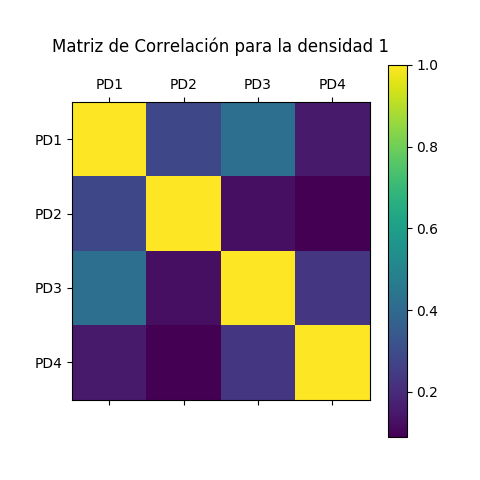
\includegraphics[scale=0.5]{correlacionD1.jpg}
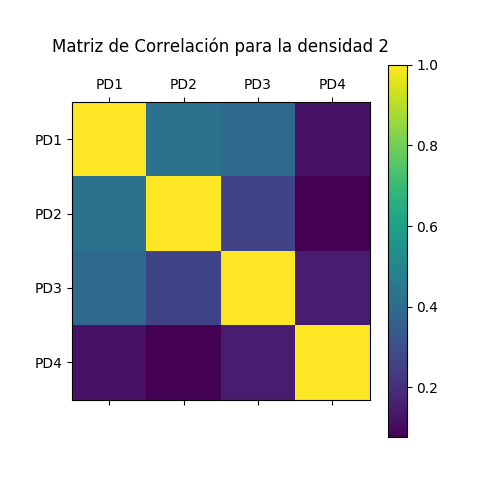
\includegraphics[scale=0.5]{correlacionD2.jpg} \\
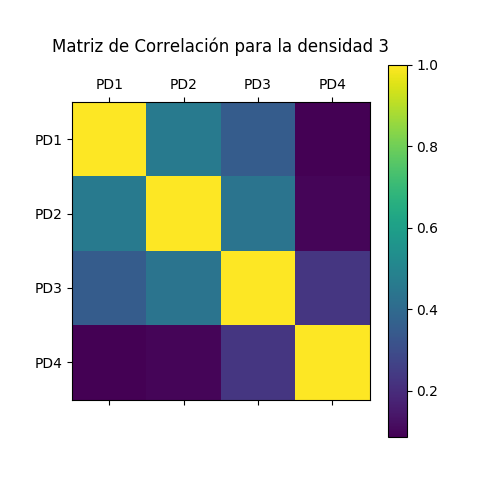
\includegraphics[scale=0.5]{correlacionD3.jpg}

Tomando en cuenta los estadísticos básicos de cada conjunto de datos se logra observar
que los valores de varianza para las variables PD1, PD2, PD3 y PD4 son altos, esto podría afectar
negativamente los cálculos del algoritmo de clasificación, a continuación se pueden observar los
histogramas de las variables de entrada para cada densidad:

\begin{center}
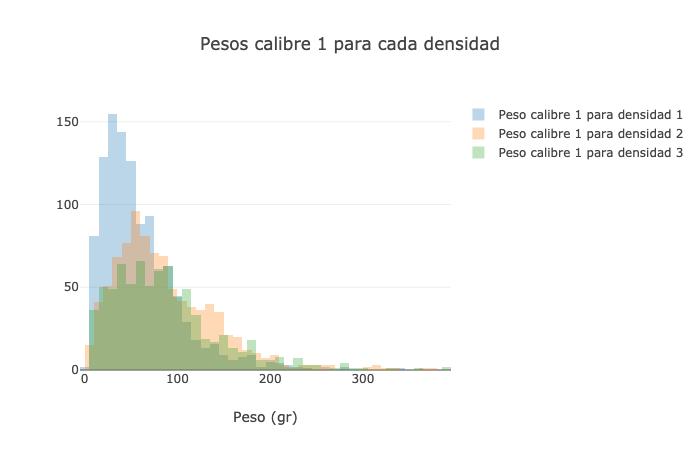
\includegraphics[scale=0.6]{PD1.png} \\
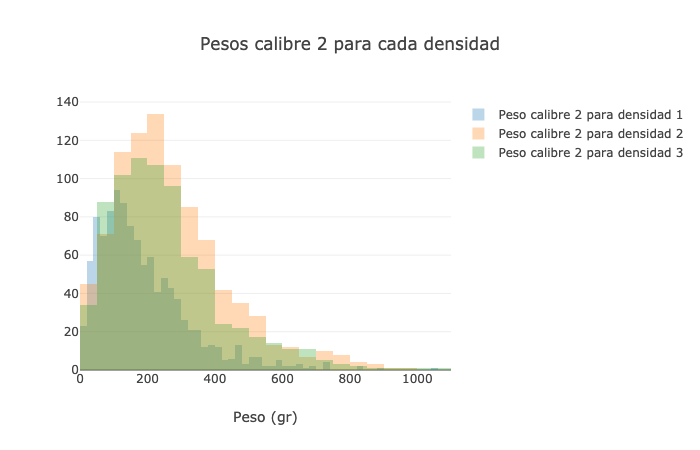
\includegraphics[scale=0.6]{PD2.png} \\
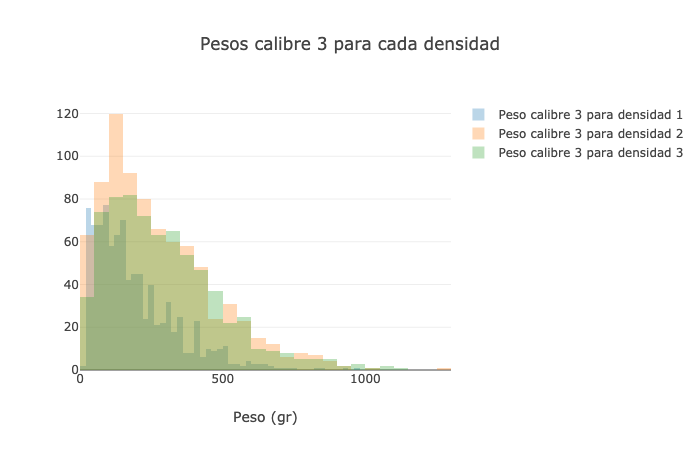
\includegraphics[scale=0.6]{PD3.png} \\
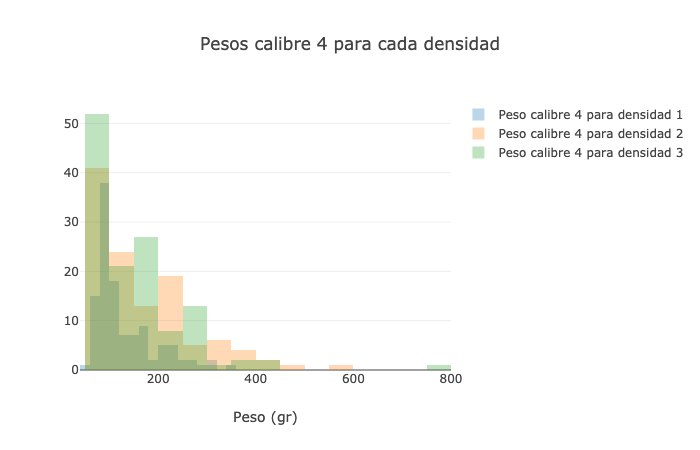
\includegraphics[scale=0.6]{PD4.png}
\end{center}

Los histogramas permiten observar que la distribución de los datos de entrada se asemeja a
una curva normal, lo que ayuda a inferir que se debe emplear el método gaussiano de
Bayes Naive para realizar su clasificación.\\\\

\noindent
\textbf{Verificación de la calidad de los datos.}\\

Luego de revisar los valores de los datos se determinó que no era necesaria la estandarización
de los mismos porque todos se encuentran en el mismo rango en cuanto a valor y en la misma unidad
de peso que es gramos (gr); No hay valores faltantes, es decir, el set de datos está completo.

\section{Preparación de datos}

\noindent
\textbf{Selección de datos.}\\

Los datos disponibles son densidad, PD1, PD2, PD3, PD4, X y Y, sin embargo, las coordenadas de las
plantas no son un dato relevante para la clasificación que se realizó porque la misma busca determinar
la densidad solo a partir de los pesos frescos por calibre, por lo tanto se excluyeron del set de datos.

\noindent
\textbf{Limpieza de los datos.}\\

No fue necesario realizar una limpieza de datos considerando la calidad de los mismos.\\

\noindent
\textbf{Estructuración de los datos.}\\

No es necesario calcular atributos derivados para realizar la clasificación; No se debe realizar
una normalización de índices porque los valores de entrada se encuentran en la misma escala y unidad,
tampoco en necesaria una normalización de puntuaciones porque se cambiaría el patron de los datos.\\

\noindent
\textbf{Integración de los datos.}\\

La media y varianza son dos datos combinados calculados a partir de los datos iniciales, estos nuevos
datos son necesarios durante el cálculo probabilístico del algoritmo clasificador y se
obtienen al principio de la ejecución llamando a la función \textbf{media\_varianza} que retorna
dos arreglos matriciales \textbf{m} y \textbf{v}, con un número de filas igual a la cantidad de clases, en este caso tres filas,
y la cantidad de columnas es igual a la cantidad de características de entrada, es decir, cuatro
para la data que se está empleando, cada campo de la matriz contiene la media o varianza (dependiendo de la
matriz que se este revisando) para esa característica y esa clase.\\

\noindent
\textbf{Formateo de los datos.}\\

Los datos de entrada se encuentran ordenados según su clase, por lo tanto deben ser desordenados
para permitir que el algoritmo de clasificación obtenga datos de cada clase para realizar los
cálculos, se desordenaron las filas de datos empleando la función \textbf{random.shuffle} del paquete
\textbf{numpy} para python.\\

\section{Modelado}

\noindent
\textbf{Técnica de modelado.}\\

El desarrollo del clasificador se realizó empleando Bayes Naive Gaussiano, luego de leer los datos se llama a la función \textbf{bayes\_naive\_gaussiano} que recibe como entrada los siguientes parámetros:
\begin{itemize}
	\item{set\_entrenamiento: es un array de numpy con las columnas número de planta, densidad, PD1, PD2, PD3, PD4, X y Y, su cantidad de filas depende de la cantidad de datos que sean destinados a formar parte del entrenamiento que es este caso en el 80\% de los datos iniciales, es decir, aproximadamente 2272 filas.}
	\item{set\_test: es un array de numpy con las columnas PD1, PD2, PD3 y PD4, su cantidad de filas depende de la cantidad de datos que sean destinados a formar parte del set de pruebas que es este caso en el 20\% de los datos iniciales, es decir, aproximadamente 567 filas.}
	\item{clases\_set\_test: es un array de numpy y cada fila representa la clase (densidad) para los datos en el set de test en el mismo número de fila, su cantidad de filas depende de la cantidad de datos que sean destinados a formar parte del set de pruebas que es este caso en el 20\% de los datos iniciales, es decir, aproximadamente 567 filas.}
\end{itemize}

Y ejecuta los siguientes pasos:
\begin{enumerate}
	\item {Realiza el cálculo de la media y varianza por cada característica y cada clase.}
	\item {Calcula la probabilidad previa para cada clase.}
	\item {Hace el cálculo de la probabilidad posterior de las características del set de pruebas para cada clase.}
	\item {Obtiene las probabilidades condicionales según el Teorema de Bayes y las predicciones.}
	\item {Realiza el análisis de los resultados empleando la curva característica operativa del receptor.}
\end{enumerate}

\noindent
\textbf{Método de evaluación de los modelos.}\\

\section{Evaluación}

\noindent
\textbf{Evaluación de los resultados.}\\

\noindent
\textbf{Proceso de revisión.}\\

\noindent
\textbf{Determinación de futuras fases.}\\